\documentclass{AsignaturaResumen}

\def\ISMAIN{1}
\SetTitulo{Tecnología enzimática}
\setabbreviationstyle[acronym]{long-short}
\makeglossaries

    % Glosario

\newglossaryentry{polimorfismo}{
    name={Polimorfismo},
    description={Existencia de dos o más variantes (alelos) de una secuencia de ADN en una población}
}
\newglossaryentry{locus}{
    name={Locus},description={Posición que ocupa un gen en el cromosoma}}
\newglossaryentry{amplicones}{
    name={Amplicones},
    description={Secuencias de ADN producidas por la amplificación de la hebra original en una \acrshort{pcr}. Se identifican como las bandas de una electroforesis en gel}
}
\newglossaryentry{sucesion microbiana}{
    name={Sucesión microbiana},
    description={Evento donde las especies de microorganismos presentes en una muestran son reemplazadas por otras}
}
\newglossaryentry{variante de secuencia}{
    name={Variante de Secuencia de Amplicón},
    description={Amplicón único de un conjunto de secuencias obtenidas en una secuenciación ya corregida}
}
\newglossaryentry{homopolimero}{
    name={Homopolímero},
    description={Secuencia repetitiva de nucleótidos (AGTGCGAT\emph{AAAA}TGCAGT, p.e.)}
}

    % Acrónimos

\newacronym{si}{SI}{Sistema Internacional}
\newacronym{iubmb}{IUBMB}{Unión Internacional de Bioquímica y Biología Molecular}

\newacronym{ros}{ROS}{especies reactivas de oxígeno}

\newacronym{pb}{pb}{pares de bases}
\newacronym{kb}{kb}{kilobases}

\newacronym{adn}{ADN}{Ácido desoxirribonucléico}
\newacronym{adnc}{ADNc}{ADN complementario}
\newacronym{dntps}{dNTPs}{desoxirribonucleótidos trifosfato}
\newacronym{ddntps}{ddNTPs}{didesoxinucleótidos}

\newacronym{adnpol}{ADNpol}{ADN polimerasa}

\newacronym{pcr}{PCR}{Reacción en Cadena de la Polimerasa}
\newacronym{rapd}{RAPD}{ADN Polimórfico Amplificado al Azar}
\newacronym{rflp}{RFLP}{Fragmentos de Restricción de Longitud Polimórfica}
\newacronym{dpcr}{dPCR}{PCR digital}
\newacronym{ngs}{NGS}{Secuenciación de Nueva Generación}
\newacronym{smrt}{SMRT}{Secuenciación en Tiempo Real de Molécula Única}

\newacronym{ccs}{CCS}{Lecturas de Consenso Circular}
\newacronym{asv}{ASV}{Variante de Secuencia de Amplicón}

\newacronym{iqi}{IQI}{Índice de Calidad Infaunal}

\newacronym{sds}{SDS}{dodecilsulfato sódico}
\newacronym{dms}{DMS}{dimetilsulfato}
\newacronym{ctab}{CTAB}{bromuro de cetiltrimetilamonio}

\begin{document}

    \frontmatter

\Portada
\Indices

    \mainmatter


\part{Fundamentos de biocatálisis}

    \chapter{Estructura de las enzimas} 
Toda reacción química toma un tiempo dado en ocurrir, sin embargo, existen sustancias capaces de acelerar la velocidad de estas reacciones, estas sustancias son conocidas como \emph{catalizadores}. Para la vida en la Tierra este tema de la velocidad de las reacciones químicas es de suma importancia. Tomemos como ejemplo, la degradación del peróxido de hidrógeno (\ce{H2O2}) en agua y oxígeno: 

\begin{equation*}
    \ce{H2O2 -> 2H2O + O2}
\end{equation*}

Esta reacción puede ocurrir de manera autónoma, sin ayuda externa de energía o sustancias extra, sin embargo, tomaría un tiempo considerable en ocurrir de esta forma. Dado que el \ce{H2O2} es un compuesto oxidante, puede ser dañino para los seres vivos, es necesario acelerar su reacción de degradación para deshacerse de él lo más rápido posible, o sea, necesitan un catalizador. Afortunadamente los seres vivos han desarrollado sus propios catalizadores, las \emph{enzimas}. Por ejemplo, el uso de la enzima como catalasa puede hacer que la degradación de peróxido mencionada antes ocurra hasta 1000 millones de veces más rápido\citep{mathewsBioquimica2002}, y así como esta enzima para esta reacción concreta, los seres vivos utilizan estas enzimas para hacer que sus procesos bioquímicos se desarrollen de manera adecuada.

Así pues, las enzimas se pueden definir como \emph{catalizadores biológicos}, moléculas que utilizan los seres vivos para acelerar reacciones químicas.

Más específicamente hablando, las enzimas son \emph{proteínas}. Conviene pues recordar la estructura básica de las proteínas, pues muchos de los aspectos que se estudian acerca de las enzimas, así como los procesos que se siguen para su aislamiento y uso, derivan de las características bioquímicas de las proteínas en general.



\section{Recordando la estructura de las proteínas}\label{sec:estructura_proteica_de_las_enzimas}

Las proteínas son \emph{polímeros}, o sea, sustancias compuestas de pequeñas moléculas ``base'' que se ensamblan entre sí. las cuales son llamados \emph{monómeros}. En el caso de las proteínas, sus monómeros son los \emph{aminoácidos}. Aspectos como la cantidad, el tipo y el orden de los aminoácidos de una proteína definen las características que esta tendrá.

Podemos dividir la \emph{estructura general} de un aminoácido en un \emph{carbono central alfa} ($\alpha$) del cual se desprenden 3 grupos: el grupo amino (\ce{NH2}), el grupo carboxilo (\ce{COOH}) y la cadena lateral (R). 

Los \emph{grupos amino y carboxilo} son grupos funcionales\footnote{O sea, capaces de reaccionar} a través de los cuales los aminoácidos se pueden unir entre sí. Tal unión entre aminoácidos por medio de tales grupos se llama \emph{enlace peptídico}. Estos grupos dotan además a los aminoácidos de un \emph{caracter anfotérico}, o sea, que puede actuar tanto como ácido y como base, esto porque cada grupo se ioniza de manera diferente dependiendo el pH del medio. 

Por otro lado, la \emph{cadena lateral} es una cadena de átomos la cual es diferente para cada aminoácido, por lo que las características de cada cadena \emph{varían entre aminoácidos}.

\marginpar{\begin{minipage}{\marginparwidth}\begin{figure}[H]\centering
    \begin{subfigure}{\marginparwidth}\centering
        {\chemfig{H-[7]{\color{blue}N}(-[5]H)-C(-[2]{\color{green}R})-C(=[1]{\color{red}O})-[7]{\color{red}OH}} \par}
        \caption{Estructura general de un aminoácido}
        \label{fig:estructura_aminoácido_general}
    \end{subfigure}
    
    \vspace{2em}
    
    \begin{subfigure}{\marginparwidth}\centering
        {\chemfig{H-[7]{\color{blue}N}^{+}(-[5]H)(-[4]H)-C(-[2]{\color{green}R})-C(=[1]{\color{red}O})-[7]{\color{red}OH}} \par}
        \caption{Forma catiónica (+) de un aminoácido, producto de un ambiente ácido}
        \label{fig:estructura_aminoácido_acido}
    \end{subfigure}
    
    \vspace{2em}
    
    \begin{subfigure}{\marginparwidth}\centering
        {\chemfig{H-[7]{\color{blue}N}(-[5]H)-C(-[2]{\color{green}R})-C(=[1]{\color{red}O})-[7]{\color{red}O}^{-}} \par}
        \caption{Forma aniónica (-) de un aminoácido, producto de un ambiente básico}
        \label{fig:estructura_aminoácido_básico}
    \end{subfigure}
    
    \vspace{10pt}
    \rule{\marginparwidth}{0.5pt}
    \caption{Estructura de un aminoácido y sus variaciones}
\end{figure}\end{minipage}}

Así pues, las proteínas son una \emph{cadena de aminoácidos} unidos entre sí por enlaces peptídicos. Sin embargo, esta cadena no se mantiene com una simple linea recta, sino que \emph{se pliega sobre sí misma}, como si se tratara de unos audífonos con cable o unas agujetas. Estos pliegues no ocurren al azar, sino que son resultado de las \emph{interacciones de atracción o repulsión} entre los propios aminoácidos de la cadena, interacciones las cuales provienen de los átomos presentes en la cadena lateral de cada aminoácido. Un ejemplo característico es el de la cisteína, un aminoácido que cuenta con un grupo tiol (\ce{-SH}) en su cadena lateral y que puede formar enlaces disulfuro (\ce{R-S-S-R}) con otras cisteinas presentes en la cadena de aminoácidos. Estos enlaces, como cualquier otro tipo de enlace, están sujetos a las condiciones del medio, tales como su pH, temperatura, etcétera.

De todo lo anterior, lo \emph{esencial} a tener en cuenta al estudiar enzimas es que su estructura y su funcionamiento se derivan de los \emph{aminoácidos que la componen} y la \emph{integridad de sus enlaces}. El conocer su composición de aminoácidos es útil para predecir su plegamiento o identificar los aminoácidos clave involucrados en las reacciones, mientras que cuidar la integridad de sus enlaces es de suma importancia para que las enzimas no sufran ``daños'' que puedan reducir su efectividad para acelerar reacciones.

\section{Morfología de las enzimas}

Como se dijo antes, las enzimas con catalizadores biológicos que aceleran la velocidad de una reacción. Un aspecto clave de esto es que las enzimas cuentan con una \emph{alta especificidad}, o sea, que cada enzima actua de manera óptima sobre un \emph{sustrato específico} y lleva a cabo una \emph{reacción específica}. Si bien algunas enzimas son más flexibles y pueden actuar sobre varios sustratos, generalmente funcionan de manera óptima sobre uno en específico. Cual sea el caso, esta especificidad de las enzimas se origina en el \emph{centro de fijación del sustrato}, el cual es el lugar de la enzima donde el sustrato se va a unir. En este sitio se encuentran varios aminoácidos cuyas cadenas laterales están libres, y son estas cadenas las que forman un enlace con el sustrato y lo fijan a la enzima para que la catálisis pueda llevarse a cabo. Cuáles aminoácidos están presentes en tal sitio es lo que determina a qué sustrato se puede o no unir la enzima.

Una convención común a tener en cuenta antes de avanzar es que esas \emph{cadenas laterales libres} de los aminoácidos que componen a las enzimas (y a las proteínas en general) son más comunmente llamadas \emph{residuos}.

El lugar donde la catálisis se lleva a cabo se conoce como \emph{sitio activo}, y tal catálisis es llevada a cabo de igual manera por ciertos residuos presentes ahí. A estos residuos se les da el nombre de \emph{residuos catalíticos}.

\begin{figure}\centering
    \resizebox{\linewidth}{!}{\begin{tikzpicture}
\coordinate (sitio alosterico) at (1.75,1.5);
\coordinate (centro de fijacion 1) at (8,7);
\coordinate (centro de fijacion 2) at (8,5.5);
\coordinate (sitio activo) at (10,4.5);
\coordinate (centro de fijacion 3) at (12,5.5);
\coordinate (centro de fijacion 4) at (12,7);

\draw[line width=1pt] (0,0) 
    to[out=90,in=260] (sitio alosterico)
    to[out=80,in=260] (1,3)
    to[out=90,in=180] (centro de fijacion 1)
    to[out=0,in=90] (centro de fijacion 2)
    to[out=270,in=180] (sitio activo) 
    to[out=0,in=270] (centro de fijacion 3)
    to[out=90,in=180] (centro de fijacion 4)
    to[out=0,in=90] (20,0)
    to cycle;

\node[draw, anchor=north, inner sep=0.75em, align=center, font=\sffamily\large, yshift=-10pt] (sitio activo etiqueta) at (sitio activo.south) {Sitio activo};
\node[draw, anchor=west,  inner sep=0.75em, align=center, text width=4.25em, font=\sffamily\small, xshift=1em] (sitio alosterico etiqueta) at (sitio alosterico.west) {Sitio alostérico};
\node[draw, dashed, rounded corners=4pt, inner sep=0.5em, align=center, text width=6em, fill=white, font=\sffamily\footnotesize] (cambio conformacional) at (6.5,1.5) {Cambio conformacional};

\draw[dashed] (sitio alosterico etiqueta.east) to[out=0,in=180] (cambio conformacional.west);
\draw[-Stealth, dashed] (cambio conformacional.east) to[out=0,in=-90] (sitio activo etiqueta.south);

\node[draw, circle, font=\sffamily, xshift=-3cm] (ligando) at (sitio alosterico) {Ligando};
\draw[-Stealth, dashed] (ligando.east) --++ (1.5,0);

\node[draw, fill=white, circle, line width=0.5pt, node font=\sffamily, xshift=-1cm, yshift=2cm] (sustrato) at (centro de fijacion 1) {Sustrato};
\node[draw, fill=white, circle, line width=0.5pt, node font=\sffamily, xshift=1cm,  yshift=2cm] (producto) at (centro de fijacion 4) {Producto};

\node[draw, align=center, text width=4.5em, font=\sffamily\footnotesize] (residuos cataliticos) at (10,6.5) {Residuos catalíticos};

\node[anchor=west, scale=0.175] (residuo1) at (centro de fijacion 2) {\chemfig{-[:-30]-[:30]*6(-=-(-OH)=-=)}};
\node[anchor=south, scale=0.175] (residuo2) at (sitio activo) {\chemfig{-[:90](-[3]CH3)-[1]CH3}};
\node[anchor=east, scale=0.175] (residuo3) at (centro de fijacion 3) {\chemfig{-[:210]-[:150]-[:210](=[:165]O)-[:255]OH}};

\draw[<-, densely dashed, line width=0.2pt] ([xshift=0.75em]residuo1.east)  to[out=0,in=270]   (residuos cataliticos);
\draw[<-, densely dashed, line width=0.2pt] ([yshift=0.75em]residuo2.north) to[out=90,in=270]  (residuos cataliticos);
\draw[<-, densely dashed, line width=0.2pt] ([xshift=-0.75em]residuo3.west) to[out=180,in=270] (residuos cataliticos);

\draw[-Stealth, dashed] (sustrato.east) to[out=0,in=135] (residuos cataliticos.north west);
\draw[-Stealth, dashed] (residuos cataliticos.north east) to[out=45,in=180] (producto.west);
\end{tikzpicture}}
    \rule{\linewidth}{0.5pt}
    \caption{Esquema general de una enzima y su funcionamiento}
    \label{fig:esquema_de_una_enzima}
\end{figure}

Un matiz importante a mencionar aquí es que el centro de fijación y el sitio activo pueden o no ser el mismo. Cuando son el mismo el proceso es sencillo: el sustrato se une a los residuos del centro de fijación y enseguida esos mismos residuos son los residuos catalíticos que llevarán a cabo la reacción. Cuando el centro de fijación y el sitio activo son diferentes, la enzima tiene que realizar un cambio en su estructura (tambien llamado cambio conformacional) para ``acercar'' el sitio activo y sus residuos catalíticos al sustrato ya fijado.

La última región clave a conocer es el \emph{sitio alostérico}, el cual es una región que solo está presente en algunas enzimas, y la unión de ciertas moléculas en ella induce una amplia gama de efectos, como cambios estructurales, aumento o disminución en el rendimiento de la enzima, completa inhibición de la enzima, etcétera.

\section{Cofactores}

Algunas enzimas necesitan de moléculas extra para funcionar de manera correcta. Estas moléculas son conocidas como \emph{cofactores}. Tales cofactores pueden ser tanto moléculas orgánicas como inorgánicas. A estas enzimas que necesitan de un cofactor para funcionar se les conoce como \emph{apoenzima}, y una vez que tal apoenzima se une con su correspondiente cofactor, entonces toma el nombre de \emph{halo enzima}.
    \chapter{Clasificación de las enzimas} 
Así como existe una infinidad de reacciones químicas en el mundo, existen una infinidad de enzimas en la naturaleza. Intentar estudiarlas sin un orden claro sería todo un caos. Para evitar esto conviene tener una forma estándar de identidicar a las enzimas. 

Durante los inicios del estudio de las enzimas era común nombrarlas en base a sus \emph{características observables}. Por ejemplo, en 1932, Otto Warburg y Walter Christian aislaron una enzima a partir de levadura usada en producción de cerveza, y dado el color amarillento de tal enzima, decidieron nombrarla Enzima Amarilla\footnote{Completos genios}. Unos años después, en 1938, Erwin Haas aisló otra enzima con coloración amarilla a partir de levadura, por lo que la Enzima Amarilla de Otto y Walter pasó a llamarse la Vieja Enzima Amarilla (Old Yellow Enzima, OYE)\citep{williamsNewUsesOld2002}. Hoy día este par de enzimas son catalogadas como flavoproteínas, un amplio grupo de enzimas que utiliza FAD como cofactor, lo que le da a todas estas enzimas un color amarillo/verdoso. Intentar catalogar estas enzimas en base a su color sería claramente poco eficaz, y ejemplifica porqué utilizar características observables no es un buen método de clasificación.

Otra forma que ha sido utilizada para identificar a las enzimas han sido los \emph{nombres comunes}. Este nombre común usualmente se forma colocando primero el \emph{sustrato} sobre el que actua la enzima y luego la \emph{reacción} que lleva a cabo, añadiendo el \emph{sufijo -asa} a la reacción. Tomemos de ejemplo la \emph{NAD\textsuperscript{+} oxidorreductasa}, cuyo nombre se compone primero del sustrato, el \emph{NAD\textsuperscript{+}}, y luego la reacción, \emph{oxidorreducción}, añadiendo \emph{-asa} a al segundo término. Sin embargo, esto jamás fue un sistema estandarizado, por lo que tenemos enzimas como la aldolasa, cuyo nombre es poco descriptivo.

Con el objetivo de reducir tanta confusión, la \acrfull{iubmb}, específicamente su Comisión de Enzimas, estableció un sistema más lógico para denominar y numerar a las enzimas, y este sistema se ha convertido en el más utilizado hasta día de hoy.

Este sistema \emph{clasifica a las enzimas} primero que nada en base al \emph{tipo de reacción} que estas catalizan, lo que genera \emph{7 clases principales}:

\begin{enumerate}
    \item Oxidorreductasas
    \item Transferasas
    \item Hidrolasas
    \item Liasas
    \item Isomerasas
    \item Ligasas
    \item Translocasas\footnote{Esta una clase reciente, añadida apenas en 2018}
\end{enumerate}

Esto sigue sin ser suficiente para la enorme cantidad y variedad de enzimas que existen, por lo que cada una de estas clases se divide a su vez en subclases y subsubclases. Intentar navegar por tantos grupos distintos sería igualmente un caos sin una guía o mapa con el cual guiarse. Afortunadamente, la Comisión de Enzimas estableció también, el Número EC (o EC number), el cuales un identificador único para cada enzima que justamente sirve de guía a través de estas clases y subclases.

Si bien existen otras formas de clasificar a las enzimas, la propuesta por el \acrshort{iubmb} es la más utilizada, por lo que es la que se estudiará principalmente. 

Sin embargo, antes de avanzar es importante dejar un detalle en claro, y es que este sistema de clasificación \emph{no toma en cuenta la cadena de aminoácidos} que compone a la enzima. Tomemos de ejemplo la amilasa, una enzima encargada de hidrolizar glucosa. En el ser humano esta enzima es producida en la saliva y en el pancreas, y aunque en ambos casos llevan a cabo la misma reacción y se les da el mismo número EC, la composición de aminoácidos de cada una es algo diferente, esto porque están en lugares con características diferentes (pH diferente, por ejemplo). De igual manera, la cadena de aminoacidos de la amilasa de una persona no será exactamente igual a la de otra, así como la de un ser humano no será igual a la de otros animales. Este detalle es secundario cuando uno apenas aprende lo básico sobre enzimas, pero es bastante relevante en tareas más avanzadas, como la purificación de enzimas o la producción de enzimas recombinantes.



\section{Grupos principales de enzimas}\label{sec:clases_de_enzimas}

Como se mencionó antes, la primera división de las enzimas se da en base a la reacción que catalizan. Los nombres de estas clases son bastante autoexplicativos, pero conviene explorarlos un poco.

\subsection{Oxidorreductasas}

Estas enzimas llevan a cabo reacciones de oxido-reducción. Recordemos que estas reacciones consisten en 

    \begin{figure}[H]
    \centering
    {
    \chemnameinit{\chemfig{CH_3-C(-[6]H)(-[2]{\color{red}H})-O{\color{red}H}}}
    \schemestart
        \chemname{\chemfig{CH_3-C(-[6]H)(-[2]{\color{red}H})-O{\color{red}H}}}{\small\bfseries Etanol}
        \arrow(.base east--.base west){-U>[NAD+][NAD{\color{red}H} + {\color{red}H+}][][0.35][60]}[,2.5] 
        \chemname{\chemfig{CH_3-C(-[7]H)=[1]O}}{\small\bfseries Acetaldehido}
    \schemestop
    \chemnameinit{}
    \vspace*{1em} \par
    }
    \rule{\linewidth}{0.2pt}
    \caption[Oxidación del etanol en acetaldehido por la alcohol deshidrogenasa]{Reacción catalizada por la alcohol deshidrogenasa (EC 1.1.1.). Aquí la enzima utiliza el NAD\textsuperscript{+} como cofactor para oxidar el etanol, esto al eliminar de este 2 átomos de hidrógeno y 2 electrones, lo que transforma al etanol en acetaldehido. La alcohol deshidrogenasa está presente en nuestro hígado, y hoy día el principal uso que hacemos de ella es para el metabolismo de bebidas alcohólicas.}
    \label{fig:reaccion_alcohol_deshidrogenasa}
\end{figure}

\resumebox{dato}{\sci{Homo ebrius}}{La evolución de la enzima alcohol deshidrogenasa en humanos y otros homínidos ha sido relacionada con el inicio de consumo de frutas ligeramente fermentadas hace 100 millones de años\citep{carriganHominidsAdaptedMetabolize2015}}

\subsection{Transferasas}

Las transferasas llevan a cabo transferencias de grupos funcionales entre moléculas.

\begin{figure}[H]\centering
    {\schemestart
        \chemfig{}
    \schemestop \vspace*{1em} \par}
    \rule{\linewidth}{0.5pt}
    \caption{Eq}
    \label{fig:reaccion}
\end{figure}

\subsection{Hidrolasas}

Las hidrolasas son enzimas que llevan a cabo esciciones en las moléculas con la ayuda de moléculas de agua, las cuales sirven como receptoras o donadoras de electrones u átomos de oxígeno.

\begin{figure}[H]\centering
    {\schemestart
        \chemfig{}
    \schemestop \vspace*{1em} \par}
    \rule{\linewidth}{0.5pt}
    \caption{Eq}
    \label{fig:reaccion}
\end{figure}

\subsection{Liasas}

Las liasas realizan esciciones como las hidrolasas, sin embargo, estas hacen uso de moléculas de agua necesariamente.

    \begin{figure}[H]
    \centering
    {\chemnameinit{\chemfig{{\color{red}H}-C(=[2]O)-CH_3}}
    \schemestart
        \chemname{\chemfig{{\color{blue}^{-}OOC}-C(=[2]O)-CH_3}}{\small\bfseries Piruvato}
        \arrow(.base east--.base west){-U>[{\color{red}H}][][][0.3][60]}[,2]
        \chemfig{{\color{blue}C} | {\color{blue}O_2}}
        \+
        \chemname{\chemfig{{\color{red}H}-C(=[2]O)-CH_3}}{\small\bfseries Acetaldehido}
    \schemestop
    \chemnameinit{}
    \vspace*{1em}
    \par}
    \rule{\linewidth}{0.2pt}
    \caption[Descarboxilación del piruvato en acetaldehido por la piruvato descarboxilasa]{Reacción catalizada por la piruvato descarboxilasa (EC 4.1.1.1). Esta retira el grupo carboxilo (\ce{COOH}), reacción llamada descarboxilación y de donde proviene el nombre descarboxilasa. Tras esto un átomo de hidrógeno toma el lugar del grupo carboxilo.}
    \label{fig:reaccion_piruvato_descarboxilasa}
\end{figure}

\subsection{Isomerasas}

Las isomerasas llevan a cabo el reordenamiento de moléculas, por ejemplo, rotando sus grupos funcionales.

    \begin{figure}[H]
    \centering
    {
    \chemnameinit{\chemfig{^{-}OOC-[7]C(-[5]H)=C(-[7]{\color{red}H})-[1]{\color{blue}C}|{\color{blue}OO^{-}}}}
    \schemestart
        \chemname{\chemfig{^{-}OOC-[7]C(-[5]H)=C(-[7]{\color{red}H})-[1]{\color{blue}C}|{\color{blue}OO^{-}}}}{\small\bfseries Maleato}
        \arrow{<->>}
        \chemname{\chemfig{^{-}OOC-[7]C(-[5]H)=C(-[1]{\color{red}H})-[7]{\color{blue}C}|{\color{blue}OO^{-}}}}{\small\bfseries Fumarato}
    \schemestop
    \chemnameinit{}
    \vspace*{1em} \par}
    \rule{\linewidth}{0.2pt}
    \caption[Isomerización del maleato en fumarato por la maleato isomerasa]{Reacción catalizada por la maleato isomerasa (EC 5.2.1.1). Esta enzima lleva a cabo una reacción de isomeración, o sea, realiza un cambio en el ordenamiento de los átomos del sustrato, el maleato, y que genera un isómero del sustrato, fumarato.}
    \label{fig:reaccion_maleato_isomerasa}
\end{figure}

\subsection{Ligasas}

Las ligasas llevan a cabo la unión de moléculas.

    \begin{figure}[H]
    \centering
    {
    \chemnameinit{\chemfig{{\color{blue}^{-}OOC}-C(=[2]O)-CH_3}}
    \schemestart
        \chemname{\chemfig{^{-}OOC-C(=[2]O)-CH_3}}{\small\bfseries Piruvato}
        \+
        \chemfig{{\color{red}C} | {\color{red}O_2}}
        \arrow(.base east--.base west){-U>[ATP][ADP + Pi][][0.3][60]}[,2]
        \chemname{\chemfig{^{-}OOC-C(=[2]O)-CH_2-{\color{red}COO^{-}}}}{\small\bfseries Oxalacetato}
    \schemestop
    \chemnameinit{}
    %\vspace*{1em}
    \par
    }
    \rule{\linewidth}{0.2pt}
    \caption[Carboxilación del piruvato en oxalacetato por la piruvato carboxilasa]{Reacción catalizada por la piruvato carboxilasa (EC 6.4.1.1). En este ejemplo la enzima añade una molécula de dióxido de carbono (\ce{CO2}) a una molécula de piruvato, lo que genera oxalacetato. Este proceso de añadir un grupo carboxilo se conoce como carboxilación, y es el proceso opuesto a la descarboxilación viso en la \autoref{fig:reaccion_piruvato_descarboxilasa}. }
    \label{fig:reaccion_piruvato_carboxilasa}
\end{figure}

\subsection{Translocasas}

Este grupo, recien añadido en 2018, engloba aquellas enzimas encargadas de transportar moléculas de un medio dado a otro. Por ejemplo, las enzimas de la membrana celular que se dedican a transportar iones de un lado a otro de la membrana.

\begin{figure}[H]\centering
    {\schemestart
        \chemfig{}
    \schemestop \vspace*{1em} \par}
    \rule{\linewidth}{0.5pt}
    \caption{Eq}
    \label{fig:reaccion}
\end{figure}



\section{Número EC (EC Number)}

El \emph{número EC}, o EC number en ingles, es un código de 4 dígitos que se el asigna a cada enzima, donde cada dígito corresponde a un ``escalón''.

\begin{figure}[H]\centering
    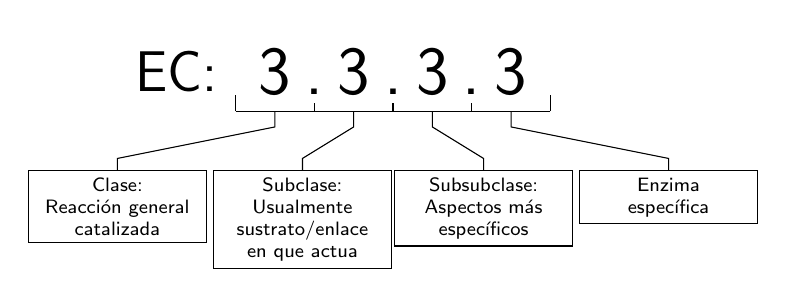
\begin{tikzpicture}
    
    \node[draw=none, node font=\huge\sffamily] at (-1.25,0) {EC:};
    \node[draw=none, node font=\Huge\sffamily] at (0,0) {3};
    \node[draw=none, node font=\Huge\sffamily] at (0.5,-0.25) {.};
    \node[draw=none, node font=\Huge\sffamily] at (1,0) {3};
    \node[draw=none, node font=\Huge\sffamily] at (1.5,-0.25) {.};
    \node[draw=none, node font=\Huge\sffamily] at (2,0) {3};
    \node[draw=none, node font=\Huge\sffamily] at (2.5,-0.25) {.};
    \node[draw=none, node font=\Huge\sffamily] at (3,0) {3};
  
    \draw (-0.5,-0.5) -- (3.5,-0.5);
    \draw (-0.5,-0.5) -- (-0.5, -0.3);
    \draw (0.5,-0.5) -- (0.5, -0.4);
    \draw (1.5,-0.5) -- (1.5, -0.4);
    \draw (2.5,-0.5) -- (2.5, -0.4);
    \draw (3.5,-0.5) -- (3.5, -0.3);

    \node[anchor=north, draw, text width=8em, align=center, node font=\scriptsize\sffamily] (clase) at (-2,-1.25) {Clase:\\Reacción general catalizada};
    \node[anchor=north, draw, text width=8em, align=center, node font=\scriptsize\sffamily] (subclase) at (0.35,-1.25) {Subclase:\\Usualmente sustrato/enlace en que actua};
    \node[anchor=north, draw, text width=8em, align=center, node font=\scriptsize\sffamily] (subsubclase) at (2.65,-1.25) {Subsubclase:\\Aspectos más específicos};
    \node[anchor=north, draw, text width=8em, align=center, node font=\scriptsize\sffamily] (enzima) at (5,-1.25) {Enzima\\específica};

    \draw (0,-0.5) --(0,-0.7) -- (-2,-1.1) -- (clase.north);
    \draw (1,-0.5) --(1,-0.7) -- (0.35,-1.1) -- (subclase.north);
    \draw (2,-0.5) --(2,-0.7) -- (2.65,-1.1) -- (subsubclase.north);
    \draw (3,-0.5) --(3,-0.7) -- (5,-1.1) -- (enzima.north);

\end{tikzpicture}
    \label{fig:ec_number}
\end{figure}

Por ejemplo, el \emph{primer dígito} corresponde a la \emph{clase principal}, las 7 que se estudiaron anteriormente (\autoref{sec:clases_de_enzimas}). El \emph{segundo dígito} corresponde a una de las \emph{subclases} existentes dentro de la clase principal las cuales describen el sustrato o enlace sobre el que actua la enzima. Lo mismo sucede con el tercer dígito que es una subclase dentro de la subclase anterior. El cuarto dígito, ahora si, es un identificador propio de cada enzima.

Este sistema se puede entender como un arbol, donde las ramas se van dividiendo en otras ramas. Aquí el número EC sirve pues como una guia sobre qué grupos seguir. Una forma visualizar esto es a través de la \textbf{\href{https://www.brenda-enzymes.org/ecexplorer2.php?browser=1}{base de datos BRENDA}}, que cuenta con un explorador de las diferentes clases de enzima.

\section{Identificador UniProt}

Como se mencionó anteriormente, la clasificación más común de enzimas se basa en la reacción que catalizan, sin embargo, esto no significa que enzimas que compartan número EC compartan también la misma cadena de aminoácidos. El \emph{identificador UniProt} es otro código el cual si que se asigna en \emph{base a la cadena de aminoácidos}.


    \chapter{Termodinámica enzimática y modelos de reacción} 
Si bien ya conocemos la estructura de una enzima y sus tipos, antes de estudiar cómo aplicarlas para catalizar reacciones es necesario aprender un detalle sobre ellas: porqué las enzimas catalizan reacciones y cómo lo hacen.

Para estudiar las razones por las cuales las enzimas tienen esta capacidad de catálisis necesitamos recordar algunos conceptos de termodinámica

\section{Termodinámica de las reacciones enzimáticas}

Los conceptos de termodinámica fundamentales para el estudio de las reacciones enzimáticas son aquellos relacionados con la primera y la segunda ley de la termodinámica. 

\subsection{Primera ley de la termodinámica}

La \emph{primera ley de la termodinámica} enuncia que \textit{``la energía ni se crea ni se destruye''}, y que la energía interna de un sistema sólo puede modificarse mediante intercambios de calor o de trabajo con el entorno.\citep{mathewsBioquimica2002,devlinBioquimica2014} Esto quiere decir que cuando ocurre una reacción química en un sistema dado, la energía que tiene ese sistema (su energía interna, representada con $E$) no va a desaparecer, sino que se transformará en otras formas de energía, específicamente calor ($q$) y/o trabajo ($w$) (\autoref{eq:cambio_de_energia_interna}).

\begin{equation}\label{eq:cambio_de_energia_interna}
    \Delta E = q - w
\end{equation}

Dado que las reacciones que estudiamos (reacciones en sistemas biológicos) ocurren a presión constante (la presión atmosférica), parte de la energía se transforma en trabajo de poco interés para nosotros. Con esto en mente, lo que nos interesa principalmente es el calor de la reacción, el cual de hecho es un aspecto fácilmente medible experimentalmente, y lo podemos definir despejando la ecuación de la siguiente manera: 

\begin{align*}
    E = q - w
    \\
    -q = -E - w
    \\
    q = E + w
\end{align*}

Dado que el trabajo ($w$) es equivalente a la presión por el volumen ($P \cdot V$), y nos interesa mantener el valor de la presión ($P$) constante, conviene expandir ese término en la ecuación:

\begin{equation}
    q = E + P \cdot V
\end{equation}

Esta nueva identidad es lo que se conoce como entalpía ($H$):

\resumebox{definicion}{Entalpía ($H$)}{Es el calor generado ($q$) en una reacción a presión constante.}

\begin{equation*}
    H = E + P \cdot V
\end{equation*}

Su cambio en una reacción ($\Delta H$) es el primer elemento a tener en cuenta para estudiar la termodinámica de las reacciones enzimáticas:

\begin{equation}
    \Delta H = \Delta E + P \cdot \Delta V
\end{equation}

\subsection{Segunda ley de la termodinámica}

La \emph{segunda ley de la termodinámica} enuncia que \textit{``la entropía de un sistema aislado tenderá a aumentar hacia un valor máximo''}\citep{mathewsBioquimica2002}.

\resumebox{definicion}{Entropía ($S$)}{La \emph{entropía} mide el grado de aleatoriedad o desorden de un sistema\citep{mathewsBioquimica2002,devlinBioquimica2014}. Se puede decir también que mide cuánto se ha dispersado la energía de un sistema, lo que hace que esta energía se encuentre menos disponible o no pueda ser utilizada}


Una forma sencilla de entender la entropía es pensar en un máquina de vapor. En estas se quema materia prima buscando utilizar la energía liberada para algo específico (calentar o mover algo, por ejemplo), sin embargo, no toda la energía liberada se aprovecha, sino que partes de esta se ``dispersan'' en el sistema, por ejemplo, en forma de calor que emanana hacia el aire, o en el roce de las piezas, etcétera. La entropía mide pues cuánto se dispersa la energía de un sistema.

\marginpar{\rule{\marginparwidth}{0.5pt}\footnotesize Los sistemas aislados no intercambian energía ni materia con su entorno.}

El aspecto clave a notar de la segunda ley es que solo se aplica de manera rigurosa a sistemas aislados, sin embargo, \emph{los sistemas biológicos no son sistemas aislados}, sino que pueden intercambiar materia y energía con el ambiente a su alrededor. Así pues, la entropía si que puede disminuir en sistemas biológicos y, como veremos adelante, es parte esencial del funcionamiento de la vida.

\section{Energía libre de Gibbs}

Para estudiar cómo fluye la energía en sistemas biológicos es necesario tener en cuenta los dos aspectos anteriormente vistos: cómo fluye la energía generada en las reacciones, la entalpía, y cómo esta energía se dispersa en el sistema, la entropía. La energía libre de Gibbs ($G$) es un valor que nos ayuda justamente a estudiar ambos aspectos de los cambios de energía en un sistema.

\begin{equation}
    \Delta G = \Delta H - T \cdot \Delta S
\end{equation}

\marginpar{\begin{minipage}{\marginparwidth}
    \begin{table}[H]
\centering

\caption{Interpretación de los posibles valores para la energía libre de Gibbs}
\label{tab:interpretacion_de_energia_libre_de_gibbs}

{\small\setstretch{1.5}\rowcolors{1}{White}{Grey}

\begin{tabular}{m{0.25\linewidth}m{0.55\linewidth}} \hline
    
    \theader{Si $\Delta G$ es:} & \theader{El proceso es:} \\ \hline
    
    Negativo & Favorecido    \\
    Cero     & En equilibro  \\
    Positivo & No favorecido \\
    
    \hline

\end{tabular}}\end{table}
\end{minipage}}

\section{Energía de activación}

Las enzimas funcionan como catalizadores al reducir la energía de activación necesaria para llevar a cabo las reacciones químicas deseadas. El estado de transición original, cuya energía de activación es alta, es remplazado por estados intermedios cuya energía de activación es menor. Las enzimas pueden generar estos estados intermedios al facilitar los cambios conformacionales de las moléculas.

\begin{figure}\centering
    \def\ProductosY{0.75}
\def\SustratoY{2.25}
\def\CatY{3.5}
\def\NoCatY{4.5}
\def\EtiquetasX{1.75}
\def\FontStyle{\sffamily\scriptsize}
\begin{tikzpicture}
    % Ejes
    \draw[-Stealth, line width=0.75pt] (0, 0) -- (0,5) node[midway, rotate=90, above=0pt, font=\sffamily\footnotesize] {Energía libre ($G$)};
    \draw[-Stealth, line width=0.75pt] (0, 0) -- (10, 0) node[midway, below=2pt, font=\sffamily\footnotesize] {Transcurso de reacción};
    % Lineas de referencia
    \draw[dashed, gray] (0,\ProductosY) -- (9.5,\ProductosY); % Productos 
    \draw[dashed, gray] (0,\SustratoY) -- (9.5,\SustratoY); % Sustrato
    \draw[dashed, red]  (0,\CatY) -- (9.5,\CatY); % Catalizada
    \draw[dashed, blue] (0,\NoCatY) -- (9.5,\NoCatY); % No catalizada
    % Etiquetas
    \node[above, inner sep=2pt, font=\FontStyle] at (\EtiquetasX,\SustratoY) {Sustrato};
    \node[above, inner sep=2pt, font=\FontStyle] at (\EtiquetasX,\ProductosY) {Productos};
    \node[above, inner sep=2pt, font=\FontStyle, red] at (\EtiquetasX,\CatY) {Reacción catalizada};
    \node[above, inner sep=2pt, font=\FontStyle, blue] at (\EtiquetasX,\NoCatY) {Reacción no catalizada};
    % Curvas de energía
    %% Catalizada
    \draw[red] 
        (0,\SustratoY) -- (2.5,\SustratoY)
        to[out=0, in=180, looseness=0.8] (5,\CatY)
        to[out=0, in=180, looseness=0.8] (8,0.75)
        -- (9,0.75);
    %% No catalizada
    \draw[blue] 
        (0,\SustratoY) -- (2.5,\SustratoY)
        to[out=0, in=180, looseness=0.8] (5,\NoCatY)
        to[out=0, in=180, looseness=0.8] (8,0.75)
        -- (9,0.75);
    % Energías de activación
    %% No catalizada
    \draw[Stealth-Stealth, blue] (7.1,\SustratoY) -- (7.1,\NoCatY)
        node[right, yshift=-0.5cm, font=\FontStyle, text=blue] {$E_{a}$ no catalizada};
    %% Catalizada
    \draw[Stealth-Stealth, red] (7.5,\SustratoY) -- (7.5,\CatY)
        node[right, midway, font=\FontStyle, text=red] {$E_{a}$ catalizada};
\end{tikzpicture}
    \caption{Diferencias de energías de activación}
    \label{fig:diferencia_de_energias_de_activacion}
\end{figure}

% En la anterior gráfica se puede observar como existe una diferencia en la energía de activación necesaria para cada reacción.

% \section{Mecanismos de catálisis}
    
%\part{Métodos de extracción de enzimas} 
%
%    \chapter{Métodos de extracción enzimática} 


\section{Fuentes de obtención}



\section{Localización celular}



\section{Métodos de extracción}



\section{Métodos de caracterización}



\section{Variables para medición de actividad enzimática}

Existen diferentes variables que se pueden medir de una reacción para de terminar su velocidad, tales como el consumo de sustrato, la producción de producto o el consumo de cofactor

Un ejemplo de medición a partir de producción de producto es el siguiente:

\begin{align*}
    H_2O_2 + OH_2 &\Longrightarrow 2H_20 + O
    \\
    O \lambda &= 440nm
\end{align*}

Para el caso de medición de consumo de cofactor, tenemos el siguiente ejemplo, donde tanto el $NAD^+$ como el $NADH$ funcionan como cofactores, y se pueden usar como elementos a medir para determinar la cinética de la reacción.

\begin{align*}
    SH_2 + NAD^{+} &\Longrightarrow NADH + H^{+} + S
    \\
    NADH \lambda &= 340nm
    \\
    \\
    SH_2 + NADH &\Longrightarrow NAD^{+} + SH_2
    \\
    NAD^{+} \lambda &= 254NM
\end{align*}

También es posible acoplar reacciones químicas a la reacción enzimática, o incluso acoplar otras reacciones enzimáticas.

\section{Métodos de medición de actividad enzimática}

Existen diversas 2 formas de medir la actividad de una enzima: de manera directa y de manera indirecta.

La primera se utiliza cuando es posible realizar una medición de alguno de los siguientes aspectos:

\begin{itemize}
    \item La disminución del sustrato conforme avanza la reacción.
    \item La acumulación del producto conforme avanza la reacción.
\end{itemize}

Por otro lado, el método indirecto se realiza cuando no puede existir una medición directa de alguno de los siguientes aspectos:

\begin{itemize}
    \item Ni sustrato
    \item Ni complejo enzima-sustrato
    \item Ni producto
\end{itemize}

Para realizar este tipo de medición se pueden realizar las siguientes operaciones:

\begin{itemize}
    \item Medir el consumo de cofactor
    \item Usar una reacción acoplada que si se pueda medir. Esta puede ser una reacción enzimática o química y necesita de especificidad y muestras de control.
\end{itemize}

\resumebox{dato}{Producción de melanina}{
    En este ejempo, se puede medir el cambio de color en una sustancia que contenga melanina (frutas o verduras, por ejemplo), y a partir de ese cambio de color determinar, de manera general y tal vez no tan exacta, si existe actividad enzimática, pues aunque las reacciones que muestran cambio de color no son enzimáticas dependen de un producto que se genera solamente por actividad de enzimas.
    \begin{align*}
        \text{Tirosina} + \text{Tirosinasa (PPO)} + O_2 + Cu^{2+} &\Longrightarrow \text{Tirosina Oxidada} + DOPA + H_2O
        \\
        \\
        DOPA + PPO + O_2 &\Longrightarrow \text{DOPA-Quinona}
        \\
        \\
        &\Longrightarrow \text{[Reacciones no enzimáticas]}
        \\
        \\
        \text{DOPA-Quinona} &\Longrightarrow \text{Dopacromo (Naranja)}
        \\
        \\
        \text{Dopacromo} &\Longrightarrow \text{5-6-hidroxi-indol (Incoloro)} + H_2O
        \\
        \\
        \text{5-6-hidroxi-indol} &\Longrightarrow \text{Indol-5-6-Quinona (Amarillo)}
        \\
        \\
        \text{Indol-5-6-Quinona} &\Longrightarrow \text{Melanocromo (Púrpura)}
        \\
        \\
        \text{N-Melanocromo} &\Longrightarrow \text{Melanina (Negra)}
    \end{align*}
}

Las mediciones también se pueden clasificar en base a qué medida de tiempo se utilize:

\begin{itemize}
    \item A tiempo final: En esta se establece un tiempo determinado y se mide unicamente en $t_i$ y $t_f$. Por ejemplo, dada una reacción con durción de 10 minutos, solo se mediría en el minuto 0 (al inicio) y al minuto 10 (al final).
    \item Cinética: En esta se establece una unidad de tiempo que determina la periodicidad con que se medirá la reacción. Por ejemplo, medir cada 30 segundos. 
\end{itemize}

\section{Papel de la espectrofotometría en la medición de actividad enzimática}

\begin{equation}
    A = \varepsilon b C
\end{equation}

Donde:

\begin{itemize}
    \item $A$ = Absorbancia (Luz absorbida)
    \item $\varepsilon$ = Absortividad (Capacidad de la sustancia para absorber luz) 
    \item $b$ = Longitud de la celda
    \item $C$ = Concentración de la solución
\end{itemize} 
%    \chapter{Purificación de enzimas} \section{Elección de la fuente}

Las fuentes de donde se puede extraer una enzima son muy variadas, pero las principales son:

\begin{itemize}
    \item Vegetales
    \item Animales
    \item Microorganismos
\end{itemize}

\section{Pasos}

\subsection{Obtención de extracto crudo (EC)}
 
En esta etapa se busca liberar la enzima del medio en el que esté, y remover restos celulares insolubles.

Técnicas de bioseparación usadas

\begin{itemize}
    \item Centrifugado
    \item Filtrado: Esta requiere de un cuidado del tamaño del poro
    \item Cromatografía
\end{itemize}

Mediciónes de importancia

\begin{itemize}
    \item Medir la actividad de la enzima
    \item Medir la concentración de la enzima
\end{itemize}

\subsection{Semipurificación - Eliminación de proteínas interferentes}

En esta etapa se busca la semipurificación, esto implica más que nada el eliminar proteínas interferentes que puedan existir en el extracto crudo previamente obtenido.

Los métodos de bioseparación usados en esta etapa suelen ser los siguientes:

\begin{itemize}
    \item Técnicas de bioseparación
    \item Precipitación
    \item Por salado: Este método se apoya del uso de sales para precipitar la proteína. La sal más recomendada es el sulfato de amonio.
    \item Por punto isoelétrico     % REVISAR
\end{itemize}

Dialisis: Este método busca separar las proteínas en base a su peso molecular. Para este método es importante cuidar los siguientes aspectos:

\begin{itemize}
    \item Mantener el extracto a baja temperatura en todo momento.
    \item Realizar cambios de agua constante para eliminar las concentraciones de sales residuales que puedan existir.
\end{itemize}

 Mediciónes de importancia
 
\begin{itemize}
    \item Medir la actividad de la enzima
    \item Medir la concentración de la enzima
\end{itemize}

\subsection{Purificación}

En esta etapa se busca, ahora sí, obtener una proteína pura.
Para esta operación se usan distintos tipos de cromatografía

Técnicas de bioseparación. Cromatografías:

\begin{itemize}
    \item Filtración en gel - Exclusión molecular
    \item Intercambio iónico
    \item Afinidad
\end{itemize}

Medición de importancia: Patrón electroforético
%    
%\part{Cinética enzimática}
%
%    \chapter{Introducción a cinética enzimática} 



% \section{Ecuación general}

La ecuación general de una reacción enzimática es la siguiente:

\begin{align*}
    \ce{E + S <=> ES -> E + P}
\end{align*}

Donde:

\begin{itemize}
    \item E = Enzima
    \item S = Sustrato
    \item ES = Complejo enzima-sustrato
    \item P = Producto
\end{itemize}

\section{Cinética química}

\begin{align*}
    \text{Reactivos} &\Longrightarrow \text{Productos} 
    \\
    \\
    \text{A} &\Longrightarrow \text{B}
    \\
    \\
    \text{Velocidad (v)} &= \frac{-d[\text{Reactivo}]}{dt}=\frac{+d[\text{Productos}]}{dt}
\end{align*}

\section{Ley de velocidad}

\begin{align*}
    V &= -\frac{dS}{dt} = \frac{dP}{dt}
    \\
    V = -\frac{dS}{dt} = \frac{dES}{dt} \ &; \ V = -\frac{dES}{dt} = \frac{dP}{dt}
\end{align*}

\begin{align*}
    [A] &= (A-A_0)
    \\
    \\
    \text{Orden O} \Longrightarrow v = \frac{-d[A]}{dt} &\rightarrow K[A]^0 \rightarrow K \rightarrow [A] = [A]_0kt
    \\
    \\
    \text{Orden 1} \Longrightarrow v = \frac{-d[A]}{dt} &\rightarrow K[A]¹
    \rightarrow ln \frac{[A]}{[A]_0} = -kt
    \\
    \\
    \text{Orden 2} \Longrightarrow v = \frac{-d[A]}{dt} &\rightarrow K[A]^2 \rightarrow \frac{1}{[A]} = \frac{1}{[A]_0} + kt
\end{align*}

\section{Órdenes de reacción ($S \longrightarrow P$)}

Las reacciones se pueden clasificar en órdenes, esto dependiendo de qué parámetros afectan su velocidad de reacción.

\begin{itemize}
    \item 0 - La velocidad depende solo de $K$.
    \item 1 - La velocidad depende de la concentración de sustrato ($[S]$) y de $K$.
\end{itemize}

La $K$ (la constante de velocidad o constante de rapidez) es un número que te dice qué tan rápida es una reacción químicamente, sin embargo, el aspecto más importante a recordar es el tema del sustrato. Las reacciones de orden 1 si aumentan su velocidad al aumentar el sustrato, las reacciones de orden 0 no.

\section{Equilibrio de reacción}

La reacción debe tener un equilibrio que favorezca la generación del complejo $E-S$ y luego el producto.
Para la formación del complejo $E-S$ existe:

\begin{itemize}
    \item $K_{1}$: El valor de equilibrio favorable
    \item $K_{2}$: El valor de equilibrio desfavorable
\end{itemize}

Esto aplica también para la reacción $ES \longrightarrow P$., y algo a tener en cuenta es que agregar enzima cambia el orden de reacción.

Un punto a tener en cuenta es que la relación entre cantidad de sustrato y cantidad de enzima cambia el orden de reacción. Como se muestra adelante (\autoref{eq:rel_concentraciones_orden}), cuando la concentración de sustrato es menor a la de enzima, el orden de reacción es de orden 1; cuando se igualan las concentraciones de ambos, se alcanza el "punto de saturación", o $V_{Max}$; y cuando la cantidad de sustrato supera la cantidad de enzima, la reacción es de orden 1.
Esto se relaciona con lo visto antes. Mientras la reacción se mantenga de orden 0, podemos agregar más sustrato para aumentar la velocidad de reacción, pero una vez se convierte en orden 1, la velocidad no aumenta, por más que agreguemos sustrato.

\begin{align*}\label{eq:rel_concentraciones_orden}
    [S] < [E] &\longrightarrow \text{Rx de orden 1}
    \\
    [S] = [E] &\longrightarrow \text{Se alcanza la saturación} = V_{max}
    \\
    [S] > [E] &\longrightarrow \text{Rx de orden 0}
\end{align*}    
%    \chapter{Factores que afectan la cinética enzimática} 


\section{Factores que afectan la velocidad de reacción}

Existen diversos parámetros que pueden afectar la velocidad con la que ocurre una reacción enzimática.

\subsection{Aspectos fisico-químicos}

Puesto que las enzimas son al final del día proteínas, debemos recordar las variables que pueden desnaturalizar una proteína, pues también afectan a las enzimas. Las principales variables son la temperatura y el pH. Hay que recordar también que estas variables cambian de enzima a enzima. Por ejemplo, mientras que cierta enzimas si pueden funcionar a temperaturas altas, existen otras que no, y viceversa. Otro punto a tomar en cuenta es que no se trata de estados de ``encendido y apagado''. Por ejemplo, una enzima que funciona a temperatura ambiente no perderá actividad de manera abrupta cuando se suba la temperatura, sino que irá perdiendo poco a poco la actividad conforme se va subiendo la temperatura.

Por todo esto, cada vez que exista una enzima que sea de nuestro interés es necesario conocer este tipo de parámetros, para poder mantener, por ejemplo, nuestro biorreactor, a las condiciones óptimas de funcionamiento de nuestra enzima.

\subsection{Inhibidores}

Existen sustancias que pueden reducir la velocidad de reacción al ``bloquear'' el funcionamiento correcto de la enzima. 

\subsection{Tipos de inhibición enzimática}

Estos se pueden clasificar de la siguiente manera:

\begin{itemize}
    \item Competitivos: Se unen al sitio catalítico y acaparan el lugar donde el sustrato entraría. Una forma de compensar la reducción de velocidad por estos inhibidores es añadir sustrato, para que ``le ganen el lugar'' al inhibidor.
    \item No competitivos: Estos se unen a otras partes de la enzima que desactivan el sitio catalítico, por lo que aunque el sustrato si se puede unir, la reacción no se lleva a cabo. Añadir sustrato no funciona aquí.
    \item 
\end{itemize}

\begin{figure}\centering
    \begin{subfigure}[t]{0.485\textwidth}
        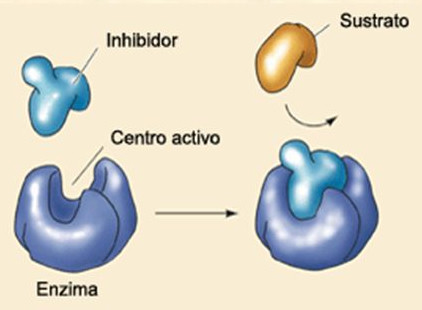
\includegraphics[width=\linewidth]{images/fig:inhibicion_competitiva}
        \caption{\textbf{Competitivo:} Aquí se muestra como el inhibidor toma lugar en el sitio activo, bloqueando la entrada del sustrato}
    \end{subfigure}
    \hfill
    \begin{subfigure}[t]{0.485\textwidth}
        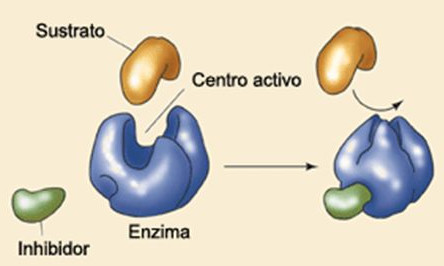
\includegraphics[width=\linewidth]{images/fig:inhibicion_no_competitiva}
        \caption{\textbf{No competitivo:} A diferencia del anterior, el sustrato si se une, pero no se lleva a cabo la reacción porque el inhibidor "bloquea" el trabajo del sitio activo.}
    \end{subfigure}
    
    \vspace*{10pt}
    \rule{\linewidth}{0.5pt}
    \caption{Tipos de inhibición enzimática}
    \label{fig:tipos_de_inhibición_enzimática_ilustrado}
\end{figure}

\marginpar{\begin{minipage}{\marginparwidth}\begin{figure}[H]\centering
    \begin{subfigure}{\linewidth}
    \centering
    \resizebox{\linewidth}{!}{
    \begin{tikzpicture}
        \draw[-Stealth, line width=0.5pt] (-5,0) -- (10,0) node[below=5pt, font=\Huge] {$\frac{1}{V}$};
        \draw[-Stealth, line width=0.5pt] ( 0,0) -- (0,10) node[xshift=-2.5em, font=\Huge] {$\frac{1}{[S]}$};
        \draw[red,  line width=0.5pt] (-2,0) -- (3,9);
        \draw[blue, line width=0.5pt] (-4,0) -- (5,8);
    \end{tikzpicture}
    }
    \rule{\linewidth}{0.2pt}
    \caption{Inhibición competitiva}
\end{subfigure}

\vspace*{10pt}

\begin{subfigure}{\linewidth}
    \centering
    \resizebox{\linewidth}{!}{
    \begin{tikzpicture}
        \draw[-Stealth, line width=0.5pt] (-5,0) -- (10,0) node[below=5pt, font=\Huge, midway] {$\frac{1}{V}$};
        \draw[-Stealth, line width=0.5pt] ( 0,0) -- (0,10) node[xshift=-2.5em, font=\Huge] {$\frac{1}{[S]}$};
        \draw[red,  line width=0.5pt] (-3.5,0) -- (3.5,8.5);
        \draw[blue, line width=0.5pt] (-1.5,0) -- (5.5,8.5);
    \end{tikzpicture}
    }
    \rule{\linewidth}{0.2pt}
    \caption{Inhibición incompetitiva}
\end{subfigure}

\vspace*{10pt}

\begin{subfigure}{\linewidth}
    \centering
    \resizebox{\linewidth}{!}{
    \begin{tikzpicture}
        \draw[-Stealth, line width=0.5pt] (-5,0) -- (10,0) node[below=5pt, font=\Huge, midway] {$\frac{1}{V}$};
        \draw[-Stealth, line width=0.5pt] ( 0,0) -- (0,10) node[xshift=-2.5em, font=\Huge] {$\frac{1}{[S]}$};
        \draw[red,  line width=0.5pt] (-2,0) -- (3,9);
        \draw[blue, line width=0.5pt] (-2,0) -- (5,8);
    \end{tikzpicture}
    }
    \rule{\linewidth}{0.2pt}
    \caption{Inhibición no competitiva}
\end{subfigure}
    \rule{\linewidth}{0.5pt}
    \caption[Tipos de inhibición enzimática graficados]{Diferencia entre los tipos de inhibición enzimática. Las gráficas representan los efectos de diferentes tipos de inhibidores en la linearización por método de Lieneawever-Burk}
    \label{fig:tipos_de_inhibicion_enzimatica}
\end{figure}\end{minipage}}

\subsubsection{Competitiva}



\subsubsection{No competitiva}



\subsubsection{Acompetitiva}



\subsubsection{Mixta}



%    \chapter{Modelos matemáticos de cinética enzimática} 



\section{Ecuación de Michaels-Menten}

\marginpar{\begin{minipage}{\marginparwidth}
    \begin{figure}[H]\centering
        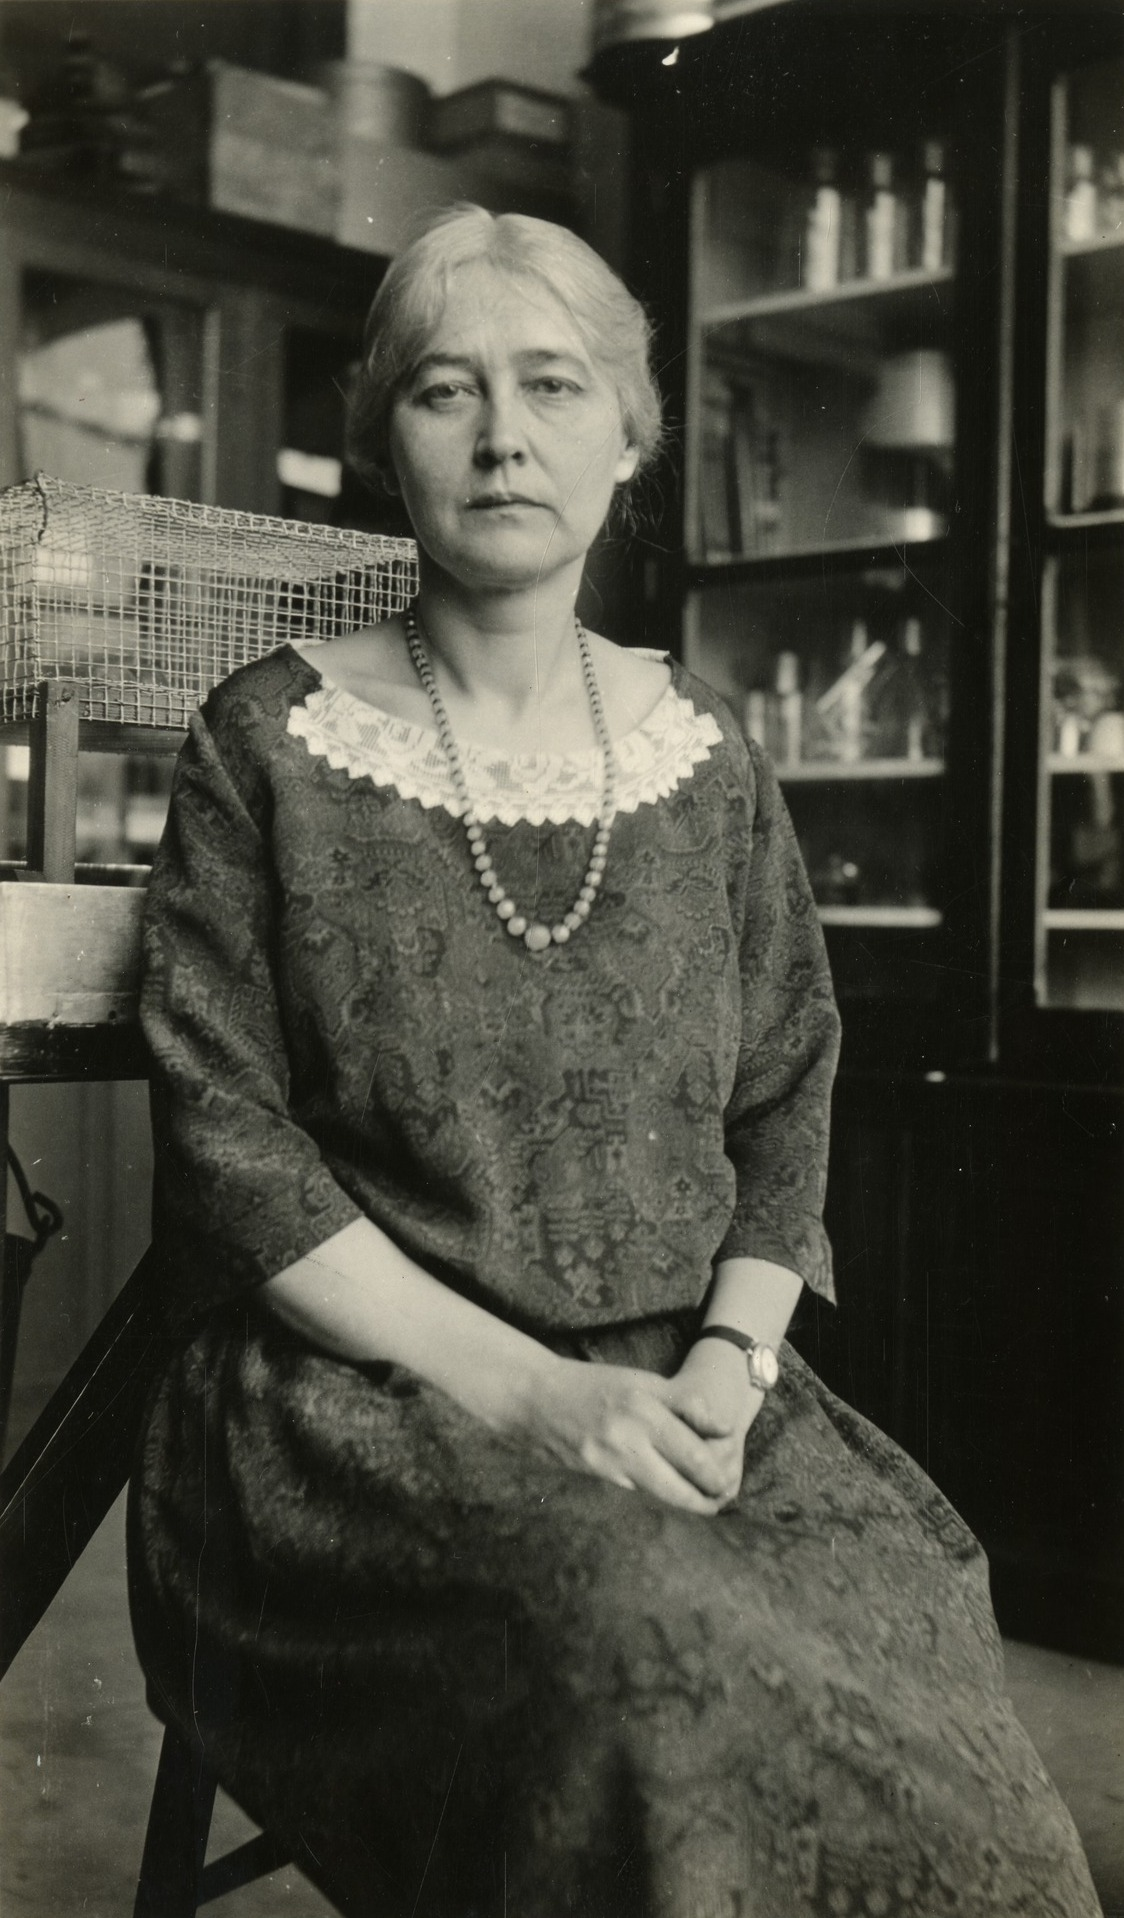
\includegraphics[width=\marginparwidth]{images/fig:leonora_menten}
        \rule{\marginparwidth}{0.5pt}
        \caption{Retrato de Leonora Menten}
        \label{fig:leonora_menten}
    \end{figure}
    \begin{figure}[H]\centering
        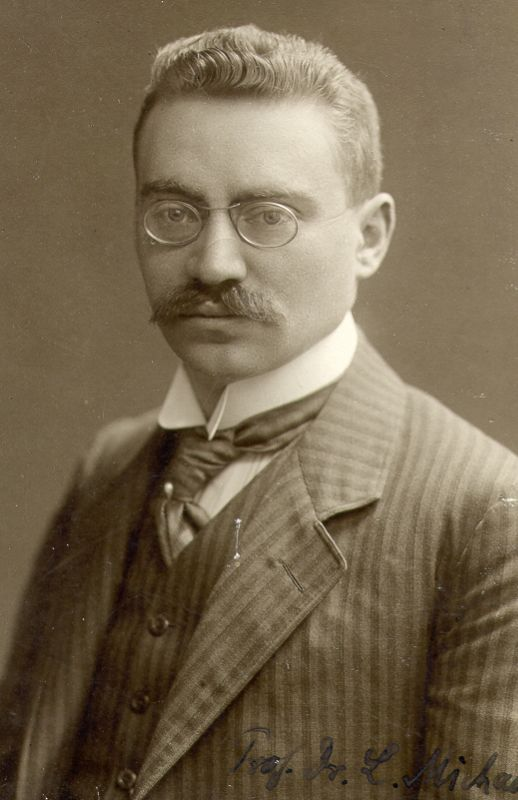
\includegraphics[width=\marginparwidth]{images/fig:leonor_michaelis}
        \rule{\marginparwidth}{0.5pt}
        \caption{Retrato de Leonor Michaelis}
        \label{fig:leonor_michaelis}
    \end{figure}
\end{minipage}}

\begin{equation}
    v = \frac{V_{max}[S]}{K_{m} + [S]}
\end{equation}

Donde:

\begin{equation*}
    Km = \text{[S] para alcanzar } \ \frac{1}{2}V_{max}
\end{equation*}

El valor de $K_{m}$ en la ecuación de Micahels-Menten es el conjunto de $K_{m}$ y $K_{cat}$

Determinar $V_{Max}$ y $K_{m}$ mediante una gráfica que tenga como ejes $[S]$ y $V$ es díficil, por lo que lo que se transforman los datos para que se pueda graficar una linea recta a partir de la cual, ahora sí, se puedan determinar los parámetros cinéticos ($V_{Max}$ y $K_{m}$) más facilmente.

Para los temas de linearización hay que primero recordar la ecuación de la recta y la forma de obtener $m$

\section{Ecuación de la recta y valor de $\mathbf{m}$}

\begin{align*}
    y &= mx+b
    \\
    m &= \frac{y_{1} - y_{0}}{x_{1} - x_{0}}
\end{align*}

Existen diferentes métodos por los cuales realizar esta transformación

\section{Valores de $\mathbf{m}$ y $\mathbf{b}$ en cada método}

Los diferentes métodos de linearización reemplazan los valores de $m$ y $b$ por ciertos parámetros cinéticos u operaciones con estos parámetros.

A su vez, es posible usar tales ecuaciones nuevas para obtener $V_{Max}$ y $K_{m}$, esto despejando la ecuación. La forma de despejarla dependerá de la formula usada, del parámetro buscado y de los datos con que ya se cuente.

En la siguiente tabla se recopila los valores que $m$ y $b$ adquieren en cada método, así como con $V_{Max}$ y $K_{m}$

    \begin{table}
\centering

\caption{Valores de $m$, $b$, $V_\text{Max}$ y $K_\text{m}$ en cada método de linearización}
\label{tab:valores_métodos_linearización}

{\small\setstretch{2}\rowcolors{1}{White}{Grey}

\begin{tabular}{M{0.275\linewidth}M{0.125\linewidth}M{0.125\linewidth}M{0.1\linewidth}M{0.15\linewidth}}\hline

    \theader{Método de linearización} & \theader{$\mathbf{m}$} & \theader{$\mathbf{b}$} & \theader{$V_\text{Max}$} & \theader{$K_\text{m}$} \\ \hline
    
    Lieneawever-Burk & $\frac{K_\text{m}}{V_\text{Max}}$ & $\frac{1}{V_\text{Max}}$          & $\frac{1}{b}$ & $V_\text{Max} \cdot m$   \\
    Eadie-Hosfstee   & K\sub{m}                          & $V_\text{Max}$                    & $b$           & $m$                           \\
    Hanes            & $\frac{1}{V_\text{Max}}$          & $\frac{K_\text{m}}{V_\text{Max}}$ & $\frac{1}{m}$ & $V_\text{Max} \cdot b$ \\
    
    \hline

\end{tabular}}\end{table}

\section{Métodos de linearización}

Aquí se desglosa en cada método cómo se cambian los valores en la ecuación de la recta por parámetros cinéticos, y cuales corresponden a cada uno.

\subsection{Lieneawever-Burk (Recíprocos)}

\begin{align*}
    y &= mx+b
    \\
    \frac{1}{V} &= \frac{K_{m}}{V_{Max}} * \frac{1}{[S]} + \frac{1}{V_{Max}}
    \\
    \\
    x = \frac{1}{[S]} \ &; \ y = \frac{1}{V}
    \\
    m &= \frac{K_{m}}{V_{Max}}
    \\
    b &= \frac{1}{V_{Max]}}
    \\
    \\
    V_{Max} &= \frac{1}{b}
    \\
    K_{m} &= m * V_{Max}
\end{align*}

\subsection{Eadie-Hosfstee}

\begin{align*}
    y &= b - mx
    \\
    V  &= V_{Max} - K_{m} * \frac{V}{[S]}
    \\
    \\
    x = \frac{V}{[S]} \ &; \ y = V
    \\
    m &= K_{m}
    \\
    b &= V_{Max}
    \\
    \\
    V_{Max} &= b
    \\
    K_{m} &= m
\end{align*}

\subsection{Hanes}

\begin{align*}
    y &= xm+b
    \\
    \frac{[S]}{V}  &= [S] * \frac{1}{V_{Max}} + \frac{K_{m}}{V_{Max}}
    \\
    \\
    x = [S] \ &; \ y = \frac{[S]}{V}
    \\
    m &= \frac{1}{V_{Max}}
    \\
    b &= \frac{K_{m}}{V_{Max]}}
    \\
    \\
    V_{Max} &= \frac{1}{m}
    \\
    K_{m} &= V_{Max} * b
\end{align*}




    \PlainGeom
    \appendix



    \backmatter

\Bibliografia
\Glosarios

\end{document}
